%論理回路とは
% =================================
% \begin{tikzpicture}[circuit logic US]

% % Inputs
% \node (A) at (0,0.1) {$A$};
% \node (B) at (0,-2.1) {$B$};

% % XOR gate (Sum)
% \node[xor gate, draw, logic gate inputs=nn] 
%   (XOR) at (3,0) {};

% % AND gate (Carry)
% \node[and gate, draw, logic gate inputs=nn] 
%   (AND) at (3,-2) {};

% % Outputs
% \node (S) at (5,0) {$S$};
% \node (C) at (5,-2) {$C$};

% % Connections
% \draw (A) -- (XOR.input 1);
% \draw (B) -- (AND.input 2);
% \draw (B) -- ++(1.5,0) |- (XOR.input 2);
% \draw (A) -- ++(2,0) |- (AND.input 1);

% \draw (XOR.output) -- (S);
% \draw (AND.output) -- (C);

% \end{tikzpicture}

\chapter{論理回路の基礎}
% =================================
\section{ブール代数と論理式}

% ---------------------------------
\subsection{論理式と論理回路について}
% ---------------------------------
論理式とは、真ならば「1」、偽ならば「0」の二値のみを扱うブール代数に基づいて論理的な演算を行うための式である。電源を入れた時を「1」、切った時を「0」に対応させるとコンピュータが扱い易いのでこの演算が採用されている。
論理回路は、入力と出力の関係を
\textbf{論理式（ブール代数）}で表すことができる。真ならば「1」、偽ならば「0」の二値のみを扱うもので、この演算方法を用いることで回路の動作を数式として扱い、設計や簡単化を行うことが可能になる。また、論理演算に対応する回路をトランジスタなどを用いて物理的に表現したものを論理ゲートと言う。例えば、論理否定はNOTゲート、論理積はANDゲート、論理和はORゲート、排他的論理和はXORゲートに対応している。

% ---------------------------------
\subsection{論理演算の記号と論理ゲートについて}
% ---------------------------------
論理演算とブール代数について
NOT（論理否定）: 条件が真であれば偽を、偽であれば真を返す。これは、条件の逆を取る演算である。
AND（論理積）: すべての条件が真である場合にのみ真を返す。例えば、AとBが両方とも真であるとき、A AND Bは真になる。
OR（論理和）: いずれかの条件が真であれば真を返す。AまたはBのいずれかが真であれば、A OR Bは真になる。
XOR（排他的論理和）：二つの値が異なる場合に真、同じ場合に偽を返す。

NOT、AND、ORゲートは次の論理式で表される。

\begin{align}
Y &= \overline{A} \\
Y &= AB \\
Y &= A + B
\end{align}

これらはすべての論理回路の基本となる。本書で用いる論理演算の記号を以下に示す。

\begin{center}
\begin{tabular}{ccc}
\toprule
論理演算 & 記号 & 意味 \\
\midrule
AND & $AB$ & A かつ B \\
OR  & $A + B$ & A または B \\
NOT & $\overline{A}$ & A の否定 \\
NAND & $\overline{AB}$ & AND の否定 \\
NOR & $\overline{A+B}$ & OR の否定 \\
XOR & $A \oplus B$ & 排他的論理和 \\
XNOR & $\overline{A \oplus B}$ & XOR の否定 \\
\bottomrule
\end{tabular}
\end{center}
\begin{itemize}
  \item 論理否定：$\overline{A}$  　例） 1→0\quad0→1
  \item 論理積：${A}\cdot{B}$    　 例）1・0\,→0\quad1・1\,→1
  \item 論理和： \,\,${A}+{B}$   　例）1+0\,→1\quad1+1\,→1\quad0+0\,→0
  \item 排他的論理和: ${A}\oplus{B}$　例）1⊕0\,→1\quad0⊕0\,→0\quad1⊕1\,→0\quad
\end{itemize}
% ---------------------------------
\subsection{論理式の簡単化}
% ---------------------------------

論理式は回路規模を小さくするために簡単化される。

よく使われる基本法則を以下に示す。

\begin{align}
A + A &= A \\
AA &= A \\
A + \overline{A} &= 1 \\
A\overline{A} &= 0 \\
A(B + C) &= AB + AC
\end{align}

これらの法則は、後述するカルノー図とも密接に関係している。


\section{論理ゲートの記号}
以下に基本的な論理回路記号を示す。真理値表とは論理式や論理回路における全ての入力の組み合わせに対して、出力に「1」と「0」を対応させた一覧表のことである。
論理式中の各演算は、そのまま回路に対応する。論理式を読み書きできることは、
論理回路設計の第一歩である。
\\
% ---------------------------------
\subsection{各種ゲートの記号と真理値表}
% ---------------------------------
\begin{center}
\begin{minipage}[t]{0.32\textwidth}
\centering
\textbf{NOT}

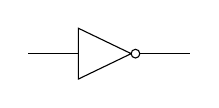
\begin{tikzpicture}[circuit logic US, scale=0.9]
\node[not gate, draw] (n) {};
\draw (n.input) -- ++(-0.7,0);
\draw (n.output) -- ++(0.7,0);
\end{tikzpicture}

\[
Y=\overline{A}
\]

\begin{tabular}{c|c}
\toprule
A & Y\\
\midrule
0 & 1\\
1 & 0\\
\bottomrule
\end{tabular}
\end{minipage}
\hfill
\begin{minipage}[t]{0.32\textwidth}
\centering
\textbf{AND}

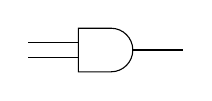
\begin{tikzpicture}[circuit logic US, scale=0.9]
\node[and gate, draw] (n) {};
\draw (n.input 1) -- ++(-0.7,0);
\draw (n.input 2) -- ++(-0.7,0);
\draw (n.output) -- ++(0.7,0);
\end{tikzpicture}

\[
Y=AB
\]

\begin{tabular}{cc|c}
\toprule
A & B & Y\\
\midrule
0 & 0 & 0\\
0 & 1 & 0\\
1 & 0 & 0\\
1 & 1 & 1\\
\bottomrule
\end{tabular}
\end{minipage}
\hfill
\begin{minipage}[t]{0.32\textwidth}
\centering
\textbf{OR}

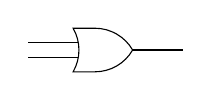
\begin{tikzpicture}[circuit logic US, scale=0.9]
\node[or gate, draw] (n) {};
\draw (n.input 1) -- ++(-0.7,0);
\draw (n.input 2) -- ++(-0.7,0);
\draw (n.output) -- ++(0.7,0);
\end{tikzpicture}

\[
Y=A+B
\]

\begin{tabular}{cc|c}
\toprule
A & B & Y\\
\midrule
0 & 0 & 0\\
0 & 1 & 1\\
1 & 0 & 1\\
1 & 1 & 1\\
\bottomrule
\end{tabular}
\end{minipage}
\end{center}

\begin{center}
\begin{minipage}[t]{0.32\textwidth}
\centering
\textbf{XOR}

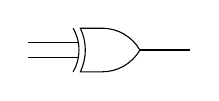
\begin{tikzpicture}[circuit logic US, scale=0.9]
\node[xor gate, draw] (n) {};
\draw (n.input 1) -- ++(-0.7,0);
\draw (n.input 2) -- ++(-0.7,0);
\draw (n.output) -- ++(0.7,0);
\end{tikzpicture}

\[
Y=A\oplus B
\]

\begin{tabular}{cc|c}
\toprule
A & B & Y\\
\midrule
0 & 0 & 0\\
0 & 1 & 1\\
1 & 0 & 1\\
1 & 1 & 0\\
\bottomrule
\end{tabular}
\end{minipage}
\hfill
\begin{minipage}[t]{0.32\textwidth}
\centering
\textbf{NAND}

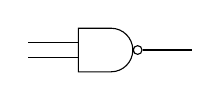
\begin{tikzpicture}[circuit logic US, scale=0.9]
\node[nand gate, draw] (n) {};
\draw (n.input 1) -- ++(-0.7,0);
\draw (n.input 2) -- ++(-0.7,0);
\draw (n.output) -- ++(0.7,0);
\end{tikzpicture}

\[
Y=\overline{AB}
\]

\begin{tabular}{cc|c}
\toprule
A & B & Y\\
\midrule
0 & 0 & 1\\
0 & 1 & 1\\
1 & 0 & 1\\
1 & 1 & 0\\
\bottomrule
\end{tabular}
\end{minipage}
\hfill
\begin{minipage}[t]{0.32\textwidth}
\centering
\textbf{NOR}

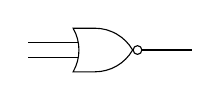
\begin{tikzpicture}[circuit logic US, scale=0.9]
\node[nor gate, draw] (n) {};
\draw (n.input 1) -- ++(-0.7,0);
\draw (n.input 2) -- ++(-0.7,0);
\draw (n.output) -- ++(0.7,0);
\end{tikzpicture}

\[
Y=\overline{A+B}
\]

\begin{tabular}{cc|c}
\toprule
A & B & Y\\
\midrule
0 & 0 & 1\\
0 & 1 & 0\\
1 & 0 & 0\\
1 & 1 & 0\\
\bottomrule
\end{tabular}
\end{minipage}
\end{center}

% ---------------------------------
\subsection{NANDゲート}
% ---------------------------------

NAND ゲートは AND ゲートの出力を否定したものである。


\[
Y = \overline{AB}
\]

NAND ゲートは \textbf{万能ゲート}であり、
NAND のみを用いてすべての論理回路を構成できる。

ド・モルガンの法則より、

\[
\overline{AB} = \overline{A} + \overline{B}
\]

と書き換えることができる。

% ---------------------------------
\subsection{NORゲート}
% ---------------------------------

NOR ゲートは OR ゲートの出力を否定したものである。

\[
Y = \overline{A + B}
\]

こちらも NAND と同様に万能ゲートである。

ド・モルガンの法則を用いると、

\[
\overline{A + B} = \overline{A}\,\overline{B}
\]

と表せる。

% ---------------------------------
\subsection{XORゲート}
% ---------------------------------

XOR は「入力が異なるときに 1 となる」論理である。

\[
Y = A \oplus B
\]

AND / OR / NOT を用いて展開すると、

\[
Y = \overline{A}B + A\overline{B}
\]

となる。



\section{真理値表とカルノー図}
% ---------------------------------
\subsection{真理値表から論理式を作る}
% ---------------------------------

真理値表から論理式を作る手順を以下の真理値表を例にとって考える。
手順は以下に示す。

\begin{enumerate}
  \item 出力が 1 となる入力の組を探す
  \item それぞれを AND 項として書き出す
  \item OR でまとめる
\end{enumerate}

\begin{center}
\begin{tabular}{ccc|c}
\toprule
A & B & C & Y \\
\midrule
0 & 0 & 0 & 0 \\
1 & 0 & 0 & 0 \\
0 & 1 & 0 & 0 \\
0 & 0 & 1 & 0 \\
1 & 1 & 0 & 1 \\
1 & 0 & 1 & 1 \\
0 & 1 & 1 & 1 \\
1 & 1 & 1 & 1 \\
\bottomrule
\end{tabular}
\end{center}

この真理値表から、
\[
\begin{aligned}
Y &= AB\overline{C} + A\overline{B}C + \overline{A}BC + ABC \\
  &= AB\overline{C} + A\overline{B}C + \overline{A}BC + (ABC + ABC + ABC) \\
  &= (AB\overline{C} + ABC) + (A\overline{B}C + ABC) + (\overline{A}BC + ABC) \\
  &= AB(\overline{C} + C) + AC(\overline{B} + B) + BC(\overline{A} + A) \\
  &= AB + AC + BC
\end{aligned}
\]
が得られる。これは、3入力多数決回路と呼ばれるものである。論理ゲートの図で表現したものを以下に示す。\\
3入力多数決回路（Majority Circuit）は，
3つの入力 $A,B,C$ のうち
\textbf{2つ以上が 1 のときに 1 を出力する}回路である。この回路は AND と OR のみで構成できる。このように、論理式を直接変形することで簡単にすることもできるが、カルノー図を使って直観的に簡単な形ににもっていくこともできる。

% ---------------------------------
\subsection{カルノー図の作成}
% ---------------------------------
カルノー図とは論理式を簡略化するために用いられる記法である。
まず，入力変数 $A,B$ を横軸，
$C$ を縦軸とする 3 変数カルノー図を作成する。
横軸はグレイコード順（00,01,11,10）で配置する。

\begin{center}
\begin{tabular}{c|cccc}
$C \backslash AB$ & 00 & 01 & 11 & 10 \\
\hline
0 & 0 & 0 & 1 & 0 \\
1 & 0 & 1 & 1 & 1 \\
\end{tabular}
\end{center}

% ---------------------------------
\subsection{グルーピング}
% ---------------------------------

カルノー図上で 1 が配置されているセルを，
2のべき乗個（1,2,4,8,...）でまとめる。

\begin{itemize}
  \item $AB=11$ の列は $C=0,1$ で 1 → $AB$
  \item $AC=11$ に対応する 2 セル → $AC$
  \item $BC=11$ に対応する 2 セル → $BC$
\end{itemize}

これにより，最小論理式が得られる。

% ---------------------------------
\subsection{最小論理式}
% ---------------------------------

\[
Y = AB + AC + BC
\]

最小論理式とは最も簡単にかける論理式のことである。この式は，「3つのうち 2つが 1」という3入力多数決の条件をそのまま表していることが分かる。

% =================================
\section{2進数の表現}
% =================================
10進数の数の場合、一桁目は10の0乗の位、二桁目は10の1乗の位、三桁目は10の2乗の位・・・と対応して考えることができる。同様に2進数の数の場合、一桁目は2の0乗の位、二桁目は2の1乗の位、三桁目は2の2乗の位・・・と対応して考えることができる。\\
例)\quad$(2)_{10} \,→\, (10)_2$\quad\,\,$(11)_{10}\,→\, (1011)_2$\quad\,\,$(35)_{10}\,→\, (100011)_2$
% =================================
\section{2進数の加算の基本}
% =================================
ここでは、2進数の加算を筆算で行い、
それがどのように論理演算（ブール演算）で
実現されているかを説明する。10進数の時と同様、桁毎に演算を行うが、繰り上がりに注意する必要がある。
10進数では 9+1 で繰り上がりが発生するが、
2進数では 1+1 で繰り上がりが発生する。


\[
\begin{array}{cccc}
 & 1 & 0 & 1 \\
+& 0 & 1 & 1 \\
\hline
1 & 0 & 0 & 0
\end{array}
\]

この計算は、下位ビットから順に処理されている。

% ---------------------------------
\subsection{1ビット加算の考え方}
% ---------------------------------

1ビット同士の加算を考える。
入力を $A,B$ とすると、次の 2 つの出力が必要になる。

\begin{itemize}
  \item 和（Sum）
  \item 桁上がり（Carry）
\end{itemize}

\begin{center}
\begin{tabular}{cc|cc}
\toprule
A & B & Sum & Carry \\
\midrule
0 & 0 & 0 & 0 \\
0 & 1 & 1 & 0 \\
1 & 0 & 1 & 0 \\
1 & 1 & 0 & 1 \\
\bottomrule
\end{tabular}
\end{center}

この表は、前章で説明した半加算器の真理値表と一致する。

% ---------------------------------
\subsection{ブール演算として見る加算}
% ---------------------------------

上の真理値表から、それぞれの出力は次の論理式で表される。

\begin{align*}
\text{Sum} &= A \oplus B \\
\text{Carry} &= AB
\end{align*}

すなわち、2進数の加算は
\textbf{XOR と AND の組み合わせ}として実現される。

% ---------------------------------
\subsection{桁上がりを含む加算}
% ---------------------------------

次に、桁上がりを含む 1 ビット加算を考える。
入力は $A,B$ に加えて、下位桁からの桁上がり $C_{\text{in}}$ がある。

\[
\begin{array}{cccc}
 & 1 & 0 & 1 \\
+& 0 & 1 & 1 \\
\hline
1 & 0 & 0 & 0
\end{array}
\]

右端の計算では

\[
1 + 1 = 0 \quad (\text{Carry } 1)
\]

となり、この Carry が次の桁へ渡される。

\subsection{半加算器（HA）}

半加算器は、2つの 1 ビット入力 $A,B$ を加算し，
和（Sum）と桁上がり（Carry）を出力する回路である。

\subsection*{論理演算の考え方}

\begin{itemize}
  \item 和（Sum）は，$A$ と $B$ が異なるときに 1
  \item 桁上がり（Carry）は，$A$ と $B$ が両方 1 のときに 1
\end{itemize}

よって，論理式は次のようになる。

\begin{align*}
\text{Sum} &= A \oplus B \\
\text{Carry} &= AB
\end{align*}

\subsection*{論理ゲート図}
\begin{center}
\usetikzlibrary{circuits.logic.US}
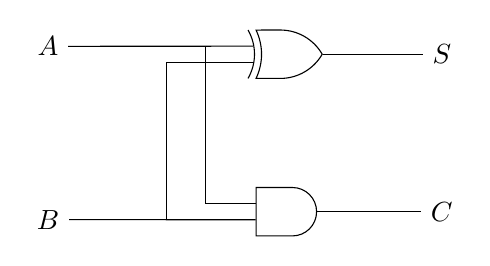
\begin{tikzpicture}[circuit logic US]

% Inputs
\node (A) at (0,0.1) {$A$};
\node (B) at (0,-2.1) {$B$};

% XOR gate (Sum)
\node[xor gate, draw, logic gate inputs=nn] 
  (XOR) at (3,0) {};

% AND gate (Carry)
\node[and gate, draw, logic gate inputs=nn] 
  (AND) at (3,-2) {};

% Outputs
\node (S) at (5,0) {$S$};
\node (C) at (5,-2) {$C$};

% Connections
\draw (A) -- (XOR.input 1);
\draw (B) -- (AND.input 2);
\draw (B) -- ++(1.5,0) |- (XOR.input 2);
\draw (A) -- ++(2,0) |- (AND.input 1);

\draw (XOR.output) -- (S);
\draw (AND.output) -- (C);

\end{tikzpicture}
\end{center}



\subsection*{真理値表}

\begin{center}
\begin{tabular}{cc|cc}
\toprule
A & B & Sum & Carry \\
\midrule
0 & 0 & 0 & 0 \\
0 & 1 & 1 & 0 \\
1 & 0 & 1 & 0 \\
1 & 1 & 0 & 1 \\
\bottomrule
\end{tabular}
\end{center}

\subsection{全加算器（FA）}

全加算器は，入力 $A,B$ に加えて，
下位桁からの桁上がり $C_{\text{in}}$ を含めて加算を行う回路である。

\subsection*{論理演算の考え方}

\begin{itemize}
  \item 和（Sum）は，3入力のうち 1 の個数が奇数のときに 1
  \item 桁上がり（Carry）は，2つ以上が 1 のときに 1
\end{itemize}

これより，論理式は次のように表される。

\begin{align*}
\text{Sum} &= A \oplus B \oplus C_{\text{in}} \\
\text{Carry} &= AB + C_{\text{in}}(A \oplus B)
\end{align*}

\subsection*{論理ゲート図}

\begin{center}
  \begin{tikzpicture}[circuit logic US]
    % Half adder 2
    \draw (4,1) node[xor gate] (xor2) {};
    \draw (xor2)+(0,1) node[and gate] (and2) {};

    % Half adder 1
    \draw (and2.input 1)+(-2,0) node[xor gate] (xor1) {};
    \draw (xor1)+(0,1) node[and gate] (and1) {};

    % Carry
    \draw ($0.5*(and1)+0.5*(and2)+(3,0)$) node[or gate] (or) {};

    % connection between AND1 and XOR1
    \draw (and1.input 1) to ++(-0.70,0) node [branch] {} |- (xor1.input 1);
    \draw (and1.input 2) to ++(-0.35,0) node [branch] {} |- (xor1.input 2);

    % connection between HA1 and HA2
    \draw (xor1.output) -- (and2.input 1);

    % connection between AND1 and XOR1
    \draw (xor1.output)  to ++( 0.70,0) node [branch] {} |- (xor2.input 1);
    \draw (xor2.input 2) to ++(-0.35,0) node [branch] {} |- (and2.input 2);

    % connection between AND1,2 and OR
    \draw (or.input 2) -- ++(-0.4,0) |- (and2.output);
    \draw (or.input 1) -- ++(-0.4,0) |- (and1.output);

    % outputs
     \draw (or.output) -- ++(1,0) node[right] (output) {$Carry$};
     \draw (xor2.output) -- ($($(or.output)+(1,0)$)!(xor2.output)!($(or.output)+(1,1)$)$) node[right] {$Sum$};

    % inputs
     \draw (xor2.input 2) -- ($(0,1)!(xor2.input 2)!(0,0)$) node[left] {$C_{in}$};
     \draw (and1.input 1) -- ($(0,1)!(and1.input 1)!(0,0)$) node[above] {$A$};
     \draw (and1.input 2) -- ($(0,1)!(and1.input 2)!(0,0)$) node[below] {$B$};
  \end{tikzpicture}
\end{center}

\subsection*{真理値表}

\begin{center}
\begin{tabular}{ccc|cc}
\toprule
A & B & $C_{\text{in}}$ & Sum & Carry \\
\midrule
0 & 0 & 0 & 0 & 0 \\
0 & 0 & 1 & 1 & 0 \\
0 & 1 & 0 & 1 & 0 \\
0 & 1 & 1 & 0 & 1 \\
1 & 0 & 0 & 1 & 0 \\
1 & 0 & 1 & 0 & 1 \\
1 & 1 & 0 & 0 & 1 \\
1 & 1 & 1 & 1 & 1 \\
\bottomrule
\end{tabular}
\end{center}

% =================================
\section{おまけ}
% =================================

本章では，加算器を基にした減算の方法と，
複数ビット加算における時間的な問題について解説する。

% ---------------------------------
\subsection{減算器の考え方}
% ---------------------------------

2進数の減算 $A - B$ は，
2の補数表現を用いることで加算として処理できる。

\[
A - B = A + (\overline{B} + 1)
\]

ここで，$\overline{B}$ は $B$ の各ビットを反転したものである。

この式から分かるように，
減算器は「反転器（NOT）」と「加算器」の組み合わせとして構成できる。

\subsection*{減算回路の構成}

\begin{itemize}
  \item $B$ の各ビットを NOT ゲートで反転する
  \item 初段のキャリー入力に 1 を与える
  \item あとは通常の加算器として処理する
\end{itemize}

この構成により，加算器と減算器を
同一の回路で兼用することが可能になる。

% ---------------------------------
\subsection{リップルキャリー加算器}
% ---------------------------------

複数ビットの加算は，
全加算器を桁ごとに直列接続することで実現される。
この構成を \textbf{リップルキャリー加算器} と呼ぶ。

\begin{figure}[h]
\centering
\begin{tikzpicture}
\node (fa1) {FA};
\node[right=1.2cm of fa1] (fa2) {FA};
\node[right=1.2cm of fa2] (fa3) {FA};
\node[right=1.2cm of fa3] (fa4) {FA};
\draw[->] (fa1) -- (fa2);
\draw[->] (fa2) -- (fa3);
\draw[->] (fa3) -- (fa4);
\end{tikzpicture}
\caption{リップルキャリー加算器の概念図}
\end{figure}

各桁のキャリー出力が次の桁へ順番に伝播するため，
キャリーは波（ripple）のように流れていく。

% ---------------------------------
\subsection{処理時間の問題}
% ---------------------------------

リップルキャリー加算器の最大の欠点は，
計算に時間がかかる点である。

最下位ビットで発生したキャリーは，
すべての桁を通過しなければ
最上位ビットの結果が確定しない。

そのため，ビット数が増えるほど，
遅延時間は次のように増加する。

\[
\text{遅延時間} \propto \text{ビット数}
\]

これは，高速な演算が求められる回路では
大きな問題となる。

% ---------------------------------
\subsection{高速化へのアプローチ}
% ---------------------------------

この問題を解決するために，
以下のような手法が考えられている。

\begin{itemize}
  \item キャリー先読み加算器（Carry Lookahead Adder）
  \item 桁ごとにキャリーを予測する構成
  \item 並列処理による遅延の削減
\end{itemize}

詳細な回路構成は複雑になるため本書では省略するが，
「速さ」と「回路規模」のトレードオフが存在することは
重要なポイントである。